\section{Auswertung}
\label{sec:Auswertung}
Aufgrund der zahlreichen Messwerte kann man die zeitlichen Temperaturverläufe sehr genau darstellen.
In den beiden folgenden Abbildungen sind die Temperaturen der äußeren Sensoren von 
Messing(breit)[T1], Messing(schmal)[T4] sowie Aluminium[T5] und Edelstahl[T8] gegenübergestellt, die bei der 
statischen Methode aufgenommen worden sind.
% side-by-side Gegenüberstellung der ersten beiden plots
\begin{figure}
    \centering
    \begin{subfigure}{.5\textwidth}
        \centering
        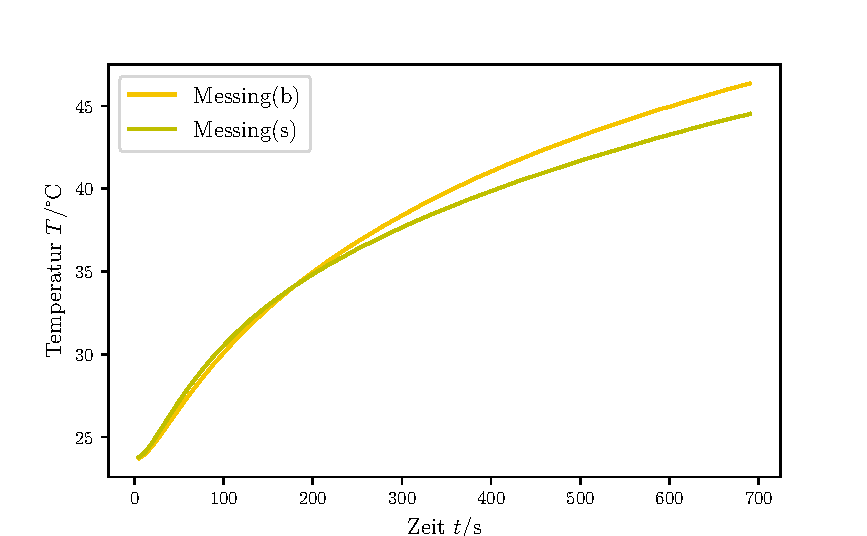
\includegraphics[max width=1.1\linewidth]{plots/plot_t1_t4.pdf}
        \caption{T1, T4.}
        \label{fig:plot_t1_t4}
    \end{subfigure}%
    \begin{subfigure}{.5\textwidth}
        \centering
        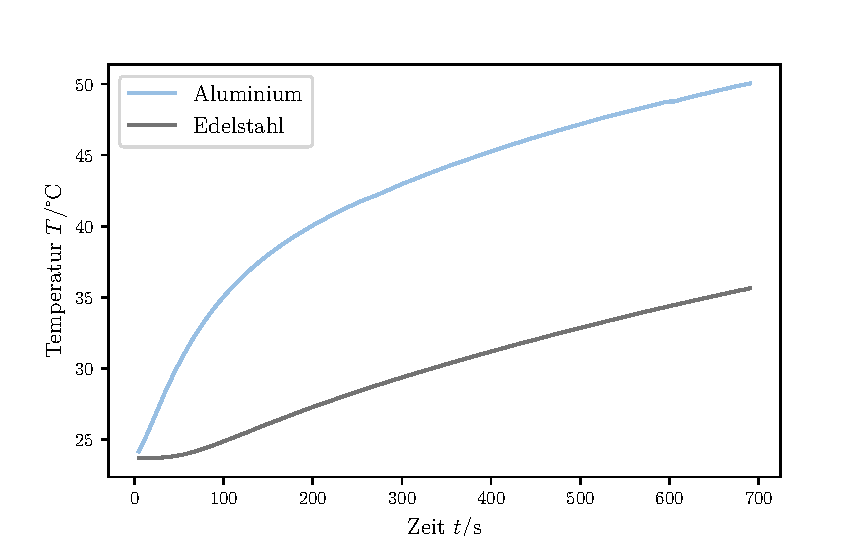
\includegraphics[max width=1.1\linewidth]{plots/plot_t5_t8.pdf}
        \caption{T5, T8}
        \label{fig:plot_t5_t8}
    \end{subfigure}
    \caption{Zeitliche Temperaturverläufe an den äußeren Sensoren}
    \label{fig:tempDiff_t1t4t5t8}
\end{figure}
Sowohl beide Messingproben als auch Aluminium weisen einen ähnlichen Funktionsgraphen auf, der augenscheinlich nur 
in horizontaler und vertikaler Skalierung variiert. 
In den etwa ersten 180 Sekunden steigt die Temperatur des schmalen Messingstabs minimal schneller an als der breite Stab. 
Danach hat der Graph des breiteren Stabs eine größere Steigung und beide Graphen steigen in gleichem Maße, um einen 
stetig wachsenden Temperaturunterschied versetzt, bis zur Endzeit.
Aluminium erreicht insgesamt die höchste Endtemperatur mit etwa $\SI{50}{\celsius}$. 
Im Gegensatz dazu steht Edelstahl: Nach einer kurzen anfänglichen Phase, in der die Temperatur kaum steigt, wächst der 
Graph nahezu linear an, was sich merklich von den Graphen unterscheidet. 
Diese besitzen vielmehr die geschwungene Form einer Wurzel- oder Logarithmus-Funktion. 

Um die Wärmeleitung besser zu untersuchen, sind hier die Endtemperaturen nach annähernd $\SI{700}{\second}$ aufgeführt:
\begin{table}
    \centering
    \caption{Äußere Temperatur nach $\SI{690}{\second}$ in $\SI{}{\celsius}$.}
    \label{tab:temp_aussen}
    \begin{tabular}{S[table-format=3.1, round-mode=places, round-precision=1] S[table-format=2.2] S[table-format=2.2] S[table-format=2.2] S[table-format=2.2]}
        \toprule
        {$t$} & {Messing(b)} & {Messing(s)} & {Aluminium} & {Edelstahl} \\
        \midrule
        690.0 & 46.36 &	44.53 &	50.04 &	35.64  \\
        \bottomrule
    \end{tabular}
\end{table}
Wie bereits erähnt hat Aluminium die höchste Endtemperatur erreicht, danach folgen der breite, der schmale Messingstab 
und Edelstahl in ebendieser Reihenfolge. 
Dementsprechend staffelt sich ebenfalls das zugehörige Maß der Wärmeleitung der einzelnen Proben. 

Nun soll für fünf verschiedene Messzeiten der Wärmestrom bestimmt werden, die sich über die Formel 
\begin{equation}
    \frac{\increment \symup{Q}}{\increment \symup{t}} = -\kappa A \frac{\increment \symup{T}}{\increment \symup{x}}
\end{equation}
berechnen lässt (vgl. dazu die Gleichung \eqref{eqn:waermemenge}). 
Hierbei gelten für Aluminium und Edelstahl ebenso die Maße der breiten Querschnittsfläche 
\begin{align*}
\symup{A}_{breit} = \SI{1.2}{\centi\m} \times \SI{0.4}{\centi\m} = \SI{0.48}{\square\centi\m},
\end{align*}
wohingegen der schmale Messingstab die Maße
\begin{align*}
\symup{A}_{schmal} = \SI{0.7}{\centi\m} \times \SI{0.4}{\centi\m} = \SI{0.28}{\square\centi\m} 
\end{align*}
erfüllt.
Bewusste Messwerte zu fünf verschiedenen Messzeiten und die sich daraus ergebenden Temperaturdifferenzen 
sind in Tabelle \ref{tab:temp_5_messwerte} und \ref{tab:tempdiff_5_messwerte} dargestellt. 
\begin{table}
    \centering
    \caption{Temperatur fünf verschiedener Messzeiten in $\si{\celsius}$.}
    \label{tab:temp_5_messwerte}
    \begin{tabular}{S[table-format=3, round-mode=places, round-precision=1] S[table-format=2.2] S[table-format=2.2] S[table-format=2.2] S[table-format=2.2] S[table-format=2.2] S[table-format=2.2] S[table-format=2.2] S[table-format=2.2]}
        \toprule
        & \multicolumn{2}{c}{Messing(breit)} & \multicolumn{2}{c}{Messing(schmal)} & \multicolumn{2}{c}{Aluminium} & \multicolumn{2}{c}{Edelstahl} \\
        \cmidrule(lr){2-3}\cmidrule(lr){4-5}\cmidrule(lr){6-7}\cmidrule(lr){8-9}
        {$t[\si{\s}]$} & {$T_{1, \text{fern}}$} & {$T_{2, \text{nah}}$} & {$T_{3, \text{nah}}$} & {$T_{4, \text{fern}}$} & {$T_{5, \text{fern}}$} & {$T_{6, \text{nah}}$} & {$T_{7, \text{nah}}$} & {$T_{8, \text{fern}}$} \\
        \midrule
        60  & 27.45 &	31.68 &	32.57 &	27.94 &  31.50 & 34.49 & 29.59 & 24.03 \\
        150 & 32.77 &	36.49 &	36.83 &	32.97 &  38.00 & 40.03 & 34.40 & 26.11 \\
        295 & 38.24 &	41.41 &	40.97 &	37.54 &  42.83 & 44.47 & 38.19 & 29.27 \\
        475 & 42.69 &	45.63 &	44.63 &	41.26 &  46.73 & 48.27 & 41.70 & 32.46 \\
        640 & 45.61 &	48.52 &	47.26 &	43.85 &  49.33 & 50.89 & 44.27 & 34.95 \\
        \bottomrule
    \end{tabular}
\end{table}

\begin{table}
    \centering
    \caption{Temperaturunterschied nah zu fern in $\si{\kelvin}$.}
    \label{tab:tempdiff_5_messwerte}
    \begin{tabular}{S[table-format=3, round-mode=places, round-precision=1] S[table-format=1.2, round-mode=places, round-precision=2] S[table-format=1.2, round-mode=places, round-precision=2] S[table-format=1.2, round-mode=places, round-precision=2] S[table-format=1.2, round-mode=places, round-precision=2]}
        \toprule
        {$t[\si{\s}]$} & {$\increment T_{Messing(breit)}$} & {$\increment T_{Messing(schmal)}$} & {$\increment T_{Aluminium}$} & {$\increment T_{Edelstahl}$} \\
        \midrule
        60  & 4.23   & 4.6299 & 2.99 &	5.559 \\
        150 & 3.7199 & 3.8599 & 2.03 &	8.29 \\
        295 & 3.1699 & 3.4299 & 1.64 &	8.91 \\
        475 & 2.94   & 3.370  & 1.54 &	9.24 \\
        640 & 2.91   & 3.4099 & 1.56 &	9.32 \\
        \bottomrule
    \end{tabular}
\end{table}

Die Werte für die materialabhängige Wärmeleitfähigkeit werden der Tabelle \ref{tab:Literaturwerte} mit den im Vorraus 
recherchierten Literaturwerten entnommen, 
der Abstand zweier Temperatursensoren ist gemäß der Messung $\increment x = \SI{3.0}{\centi\meter}$. 
Daraus ergeben sich die in Tabelle \ref{tab:Warmestrom} dargestellten Zahlenwerte für den Wärmestrom.
\begin{table}
    \centering
    \caption{Wärmestrom $\frac{\increment \symup{Q}}{\increment \symup{t}}$ in $\si{\joule\per\second}$.}
    \label{tab:Warmestrom}
    \begin{tabular}{l | S[round-mode=places, round-precision=4] S[round-mode=places, round-precision=4] S[round-mode=places, round-precision=4] S[round-mode=places, round-precision=4] S[round-mode=places, round-precision=4]}
        \toprule
        {Stoff} & {$\SI{60}{\s}$} & {$\SI{150}{\s}$} & {$\SI{295}{\s}$} & {$\SI{475}{\s}$} & {$\SI{640}{\s}$} \\
        \midrule
        Messing(breit)      & 0.758016    & 0.6666  & 0.56806 & 0.52684   & 0.52147   \\
        Messing(schmal)     & 0.483989  & 0.40349 & 0.358549 & 0.352277 & 0.35645 \\
        Aluminium           & 1.05726    & 0.71780   & 0.57990   & 0.54454   & 0.5516   \\
        Edelstahl           & 0.4092   & 0.61014  & 0.6565119 & 0.68006   & 0.68595   \\
        \bottomrule
    \end{tabular}
\end{table}

Des Weiteren sollen die an den Sensoren T7 und T8 beziehungsweise T2 und T1 gemessenen Temperaturdifferenzen in einem 
Diagramm der Zeit $t$ aufgetragen werden, also die Temperaturunterschiede an zwei verschiedenen Orten desselben Stabs, 
hier Edelstahl und Messing. 
\begin{figure}
    \centering
    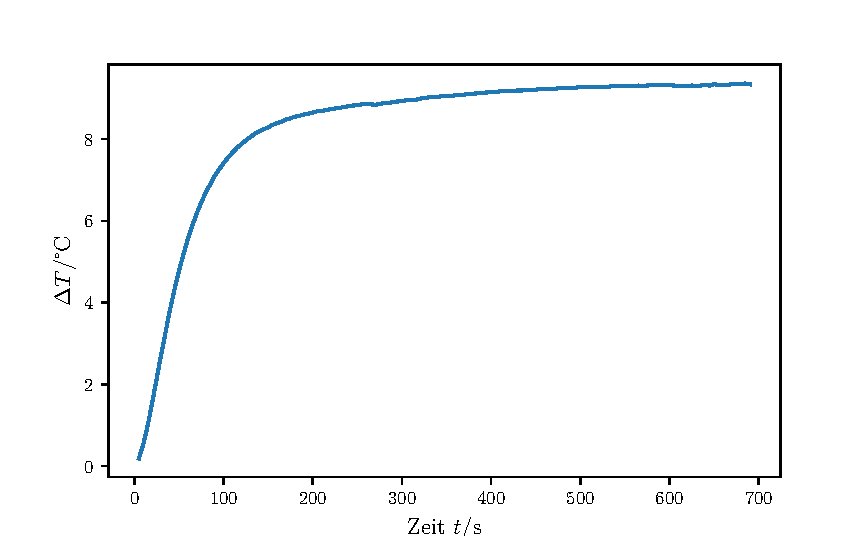
\includegraphics[max width=\linewidth]{plots/plot_tempDiff_steel.pdf}
    \caption{Temperaturdifferenz $T7 - T8$ (Edelstahl).}
    \label{fig:plot_tempDiff_t7t8}
\end{figure}

\begin{figure}
    \centering
    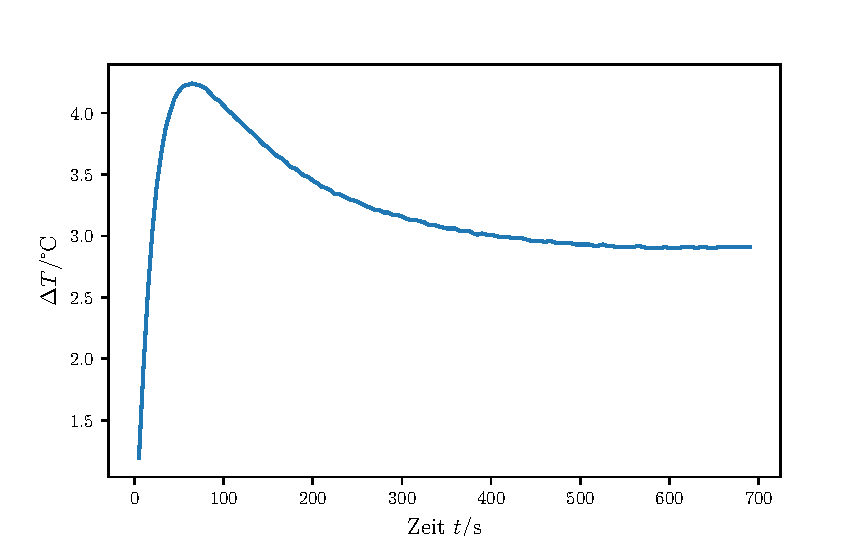
\includegraphics[max width=\linewidth]{plots/plot_tempDiff_brass_wide.pdf}
    \caption{Temperaturdifferenz $T2 - T1$ (Messing).}
    \label{fig:plot_tempDiff_t2t1}
\end{figure}
Beide Graphen haben anfänglich einen starken Anstieg, bei dem Edelstahl einen etwa doppelt so großen Wert erreicht wie Messing. 
Danach flacht die Differenz des Messings exponentiell ab, wohingegen die des Edelstahls sich asymptotisch einem Maximalwert nähert. 
Das zu Beginn starke Ansteigen indiziert das Anlegen einer dem Metall gegenüber höheren Temperatur, die zuerst am nahen 
Sensor registriert wird und erst mit einiger Zeitverzögerung an der weiter entfernten Messstelle. 
Die Temperaturdifferenz des Edelstahls steigt weiter an, das Temperaturgefälle nimmt also zu.
Dahingegen findet beim Messing ein schleichender Ausgleich der hohen Differenz statt, die Wärme verteilt sich gleichmäßiger auf dem Stab.  

\begin{table}
    \centering
    \caption{Messreihe 2 - Dynamische Methode}
    \label{tab:data2}
    \begin{tabular}{S[table-format=3.1, round-mode=places, round-precision=1] S[table-format=2.2] S[table-format=2.2] S[table-format=2.2] S[table-format=2.2] S[table-format=2.2] S[table-format=2.2] S[table-format=2.2] S[table-format=2.2]}
        \toprule
        & \multicolumn{2}{c}{Messing(breit)} & \multicolumn{2}{c}{Messing(schmal)} & \multicolumn{2}{c}{Aluminium} & \multicolumn{2}{c}{Edelstahl} \\
        \cmidrule(lr){2-3}\cmidrule(lr){4-5}\cmidrule(lr){6-7}\cmidrule(lr){8-9}
        {$t$} & {$T_{1, \text{fern}}$} & {$T_{2, \text{nah}}$} & {$T_{3, \text{nah}}$} & {$T_{4, \text{fern}}$} & {$T_{5, \text{fern}}$} & {$T_{6, \text{nah}}$} & {$T_{7, \text{nah}}$} & {$T_{8, \text{fern}}$} \\
        \midrule
        0.000 & 33.08 &	36.21 &	36.46 &	32.47 &	34.62 &	37.16 &	33.62 &	29.54 \\
        0.500 & 33.10 &	36.25 &	36.48 &	32.50 &	34.66 &	37.19 &	33.65 &	29.55 \\
        1.000 & 33.12 &	36.27 &	36.51 &	32.52 &	34.69 &	37.25 &	33.68 &	29.54 \\
        $\vdots$ & $\vdots$ & $\vdots$ & $\vdots$ & $\vdots$ & $\vdots$ & $\vdots$ & $\vdots$ & $\vdots$ \\
        882.00 & 65.16 & 65.67 & 62.65 & 61.61 & 67.34 & 65.75 & 62.62 & 50.17 \\
        \bottomrule
    \end{tabular}
\end{table}

Bei der dynamischen Messung sollen nach dem ersten Durchgang beide Temperaturverläufe der Messstellen am breiten Messingstab 
aufgetragen und die Amplituden $A_1$ und $A_2$ bei den jeweiligen Sensoren bestimmt werden. 
Dafür wurde eine Ausgleichskurve durch die Minima gezogen und die Differenz der Maxima zu dem entsprechenden Funktionswert
der Ausgleichskurve berechnet (vgl. Tabelle \ref{tab:amps_brass}). 
\begin{figure}
    \centering
    \begin{minipage}{.5\textwidth}
        \centering
        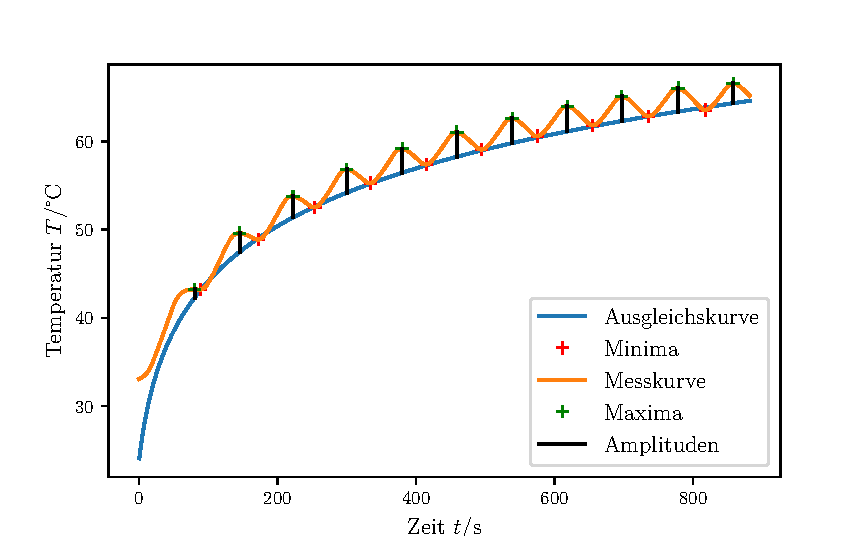
\includegraphics[max width=1.1\linewidth]{plots/amplitudes_brass_wide_far(t1).pdf}
        \caption{T1, fern.}
        \label{fig:plot_amps_t1}
    \end{minipage}%
    \begin{minipage}{.5\textwidth}
        \centering
        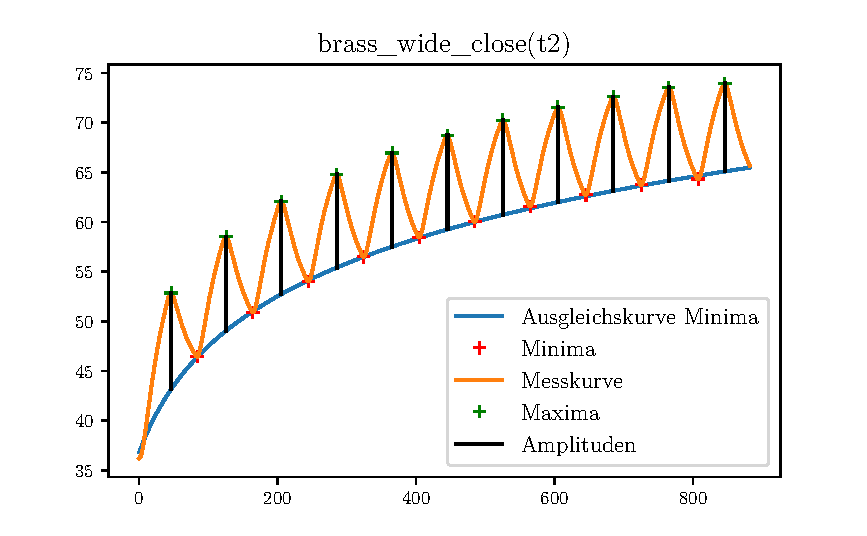
\includegraphics[max width=1.1\linewidth]{plots/amplitudes_brass_wide_close(t2).pdf}
        \caption{T2, nah.}
        \label{fig:plot_amps_t2}
    \end{minipage}
    \caption{Messwertanalyse zu Messing(breit).}
    \label{fig:plots_amps_t1_t2}
\end{figure}
\begin{table}
    \centering
    \caption{Amplituden von Messing, nah und fern, in $\si{\kelvin}$.}
    \label{tab:amps_brass}
    \begin{tabular}{S[table-format=2.1] | S[table-format=3.1] S[table-format=1.2] | S[table-format=3.1] S[table-format=1.2]}
        \toprule
         & \multicolumn{2}{c}{$\symup{Messing}_\text{nah}$} & \multicolumn{2}{c}{$\symup{Messing}_\text{fern}$} \\
        \cmidrule(lr){2-3}\cmidrule(lr){4-5}
        {$\increment t[\si{\second}]$} &{$t[\si{\second}]$} & {$\increment T[{\si{\kelvin}]}$} & {$t[\si{\s}]$} & {$\increment T[{\si{\kelvin}]}$} \\
        \midrule
        34.0   &  46.5 &	9.70 &    80.5 & 0.91 \\	
        19.5   & 126.0 &	9.47 &   145.5 & 2.11 \\		
        17.0   & 205.5 &	9.36 &   222.5 & 2.39 \\		
        14.5   & 285.5 &	9.38 &   300.0 & 2.63 \\		
        14.5   & 365.5 &	9.43 &   380.0 & 2.72 \\		
        13.5   & 445.5 &	9.46 &   459.0 & 2.78 \\		
        13.5   & 525.5 &	9.53 &   539.0 & 2.81 \\		
        13.5   & 605.0 &	9.57 &   618.5 & 2.84 \\		
        12.0   & 685.0 &	9.47 &   697.0 & 2.78 \\		
        13.5   & 765.0 &	9.40 &   778.5 & 2.65 \\
        \bottomrule
    \end{tabular}
\end{table}
Die Maxima der Temperaturkurve werden aus der Messtabelle abgelesen, da hinreichend viele Werte gegeben sind.
Zur Berechnung der Ausgleichskurve durch die Minima wird der Ansatz $\symup{f(x)}=\symup{c}*np.log(x-\symup{a})+\symup{b}$
mit den Parametern $\symup{a, b, c}$ verwendet. 
Mithilfe der numerischen Methode der kleinsten Quadrate, die durch ein entsprechendes Computerprogramm durchgeführt wird,
werden diese Parameter dann bestimmt. 
So ergibt sich für die Paramter von T1 $\symup{(a,b,c)}=(-14.69279466, -2.94742813, 9.93498876)$ und für T2 
$\symup{(a,b,c)}=(-50.49563487, -1.97913302, 9.86737879)$.
Dasselbe wird nun für die Maxima gemacht:
\begin{equation*}
\symup{T1: (a,b,c)} = ( , , ), %hier Parameter Maxima Amplituden einfügen
\symup{T2: (a,b,c)} = ( , , ).%ebenfalls einfügen
\end{equation*}
Die Differenz der abgelesenen Werte und der an der entsprechenden Stelle ausgewerteten Funktion wird berechnet. 
Mittels dieser Differenzen werden die Varianz $V(X)$ und somit die Standardabweichung $\sigma_x$ ermittelt (bei N Messwerten). 
\begin{equation*}
V(X)= \frac{1}{N} \sum_{i=0}^N \increment x_i ^2
\sigma_x = \sqrt{V(X)} 
\end{equation*}
Nun wird nach Gleichung \eqref{eqn:kappa} die Wärmeleitfähigkeit berechnet. 
Alle verwendeten Werte werden in Tabelle \ref{tab:unc_brass} dargestellt.
\begin{table}
    \centering
    \caption{Messing.}
    \label{tab:unc_brass}
    \begin{tabular}{S S S S S S S S | S S S S S S S S}
        \toprule
        \multicolumn{8}{c}{$\symup{Messing}_\text{nah}$} & \multicolumn{8}{c}{$\symup{Messing}_\text{fern}$} \\
        \cmidrule(lr){1-4}\cmidrule(lr){5-8}\cmidrule(lr){9-12}\cmidrule(lr){13-16}
        {$\increment t_min [\si{\second}]$} & {abgelesene Minima T2} & {$\symup{f_t2(t_min)}$} & {$\increment T_min$} & {$\increment t_max [\si{\second}]$} & {abgelesene Maxima T2} & {\symup{f_t2(t_max)}} & {$\increment T_max$} & 
        {$\increment t_min [\si{\second}]$} & {abgelesene Minima T1} & {$\symup{f_t1(t_min)}$} & {$\increment T_min$} & {$\increment t_max [\si{\second}]$} & {abgelesene Maxima T1} & {\symup{f_t1(t_max)}} & {$\increment T_max$}\\
        \midrule
        %hier entsprechende Zwischenwerte einfügen
        \bottomrule
    \end{tabular}
\end{table}
\begin{table}
    \centering
    \caption{Aus der jeweiligen Messdatenzeile berechnete Wärmeleitfähigkeit $\kappa$.}
    \label{tab:kappa_brass}
    \begin{tabular}{S S}
        \toprule
        {$i$} & {$\kappa_i$} \\
        \midrule
        1 &    \\  %hier berechnete werte für kappa einfügen
        2 &    \\ 
        3 &    \\ 
        4 &    \\ 
        5 &    \\ 
        6 &    \\ 
        7 &    \\ 
        8 &    \\ 
          &    \\ 
    \end{tabular}
\end{table}
Der Mittelwert der verschiedenen Werte für $\kappa$ berechnet sich durch 
\begin{equation}
\bar{x} = \frac{1}{N} \sum_{i=1}^N x_i .
\label{eqn:average}
\end{equation}
Für die Messgröße $x$ erhält man dann $x = \bar{x} \pm \sigma_x$.
Für die Wärmeleitfähigkeit des Messings ergibt sich an dieser Stelle somit $\kappa = \pm $ %hier kappa für messing einfügen inkl sigma

Dasselbe Vorgehen soll bei Aluminium durchgeführt werden:
\begin{figure}
    \centering
    \begin{minipage}{.5\textwidth}
        \centering
        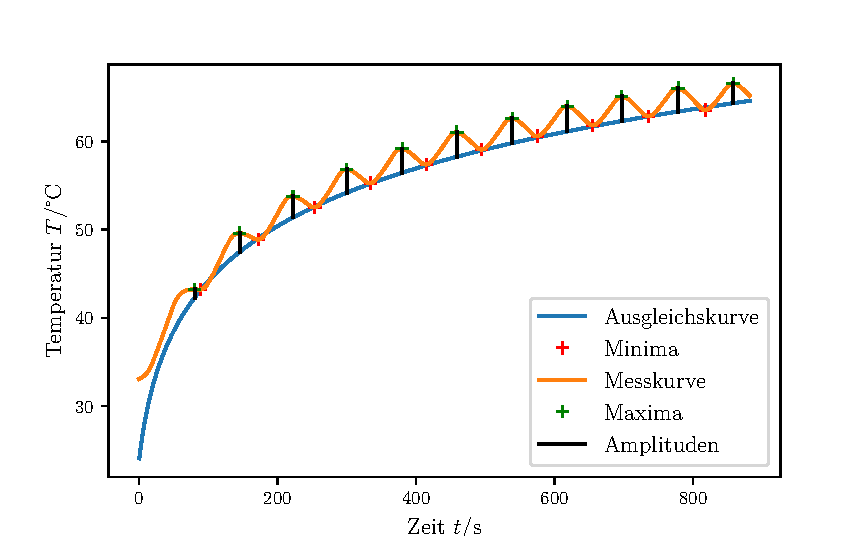
\includegraphics[max width=1.1\linewidth]{plots/amplitudes_brass_wide_far(t1).pdf} %HIER Datei für Aluminium einfügen!
        \caption{T5, fern.}
        \label{fig:plot_amps_t5}
    \end{minipage}%
    \begin{minipage}{.5\textwidth}
        \centering
        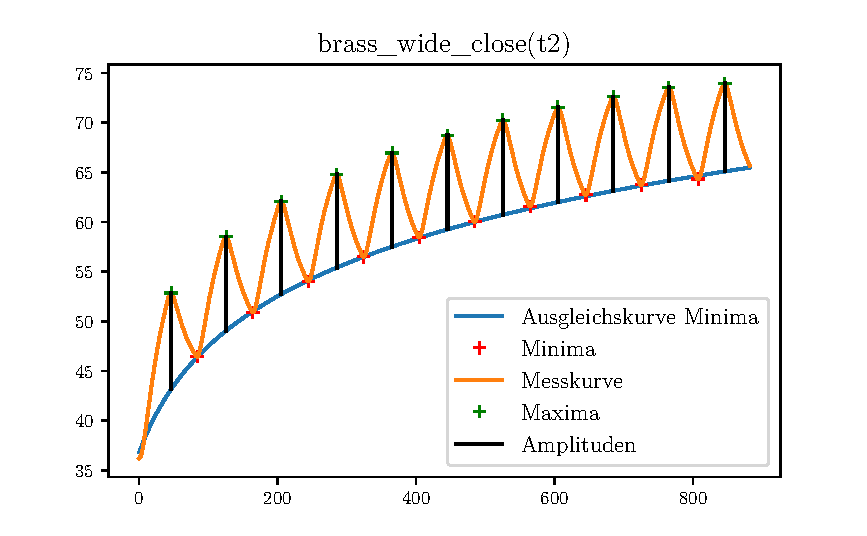
\includegraphics[max width=1.1\linewidth]{plots/amplitudes_brass_wide_close(t2).pdf} %HIER Datei Aluminium einfügen
        \caption{T6, nah.}
        \label{fig:plot_amps_t6}
    \end{minipage}
    \caption{Messwertanalyse zu Aluminium.}
    \label{fig:plots_amps_t5_t6}
\end{figure}
\begin{table}
    \centering
    \caption{Amplituden von Aluminium, nah und fern, in $\si{\kelvin}$.}
    \label{tab:amps_alu}
    \begin{tabular}{S[table-format=2.1] | S[table-format=3.1] S[table-format=1.2] | S[table-format=3.1] S[table-format=1.2]}
        \toprule
         & \multicolumn{2}{c}{$\symup{Aluminium}_\text{nah}$} & \multicolumn{2}{c}{$\symup{Aluminium}_\text{fern}$} \\
        \cmidrule(lr){2-3}\cmidrule(lr){4-5}
        {$\increment t[\si{\second}]$} &{$t[\si{\second}]$} & {$\increment T[{\si{\kelvin}]}$} & {$t[\si{\s}]$} & {$\increment T[{\si{\kelvin}]}$} \\
        \midrule
        34.0   &  46.5 &	9.70 &    80.5 & 0.91 \\	%hier die Messwerte für Aluminium einfügen (dies sind die von Messing)
        19.5   & 126.0 &	9.47 &   145.5 & 2.11 \\		
        17.0   & 205.5 &	9.36 &   222.5 & 2.39 \\		
        14.5   & 285.5 &	9.38 &   300.0 & 2.63 \\		
        14.5   & 365.5 &	9.43 &   380.0 & 2.72 \\		
        13.5   & 445.5 &	9.46 &   459.0 & 2.78 \\		
        13.5   & 525.5 &	9.53 &   539.0 & 2.81 \\		
        13.5   & 605.0 &	9.57 &   618.5 & 2.84 \\		
        12.0   & 685.0 &	9.47 &   697.0 & 2.78 \\		
        13.5   & 765.0 &	9.40 &   778.5 & 2.65 \\
        \bottomrule
    \end{tabular}
\end{table}
T5, Minima: $\symup{(a,b,c)}=()$ %Parameter für T5 und T6 einfügen
T6, Minima: $\symup{(a,b,c)}=()$
T5, Maxima: $\symup{(a,b,c)}=()$ %Parameter für T5 und T6 einfügen
T6, Maxima: $\symup{(a,b,c)}=()$

\begin{table}
    \centering
    \caption{Aluminium.}
    \label{tab:unc_alu}
    \begin{tabular}{S S S S S S S S | S S S S S S S S}
        \toprule
        \multicolumn{8}{c}{$\symup{Messing}_\text{nah}$} & \multicolumn{8}{c}{$\symup{Messing}_\text{fern}$} \\
        \cmidrule(lr){1-4}\cmidrule(lr){5-8}\cmidrule(lr){9-12}\cmidrule(lr){13-16}
        {$\increment t_min [\si{\second}]$} & {abgelesene Minima T6} & {$\symup{f_t6(t_min)}$} & {$\increment T_min$} & {$\increment t_max [\si{\second}]$} & {abgelesene Maxima T6} & {\symup{f_t6(t_max)}} & {$\increment T_max$} & 
        {$\increment t_min [\si{\second}]$} & {abgelesene Minima T5} & {$\symup{f_t5(t_min)}$} & {$\increment T_min$} & {$\increment t_max [\si{\second}]$} & {abgelesene Maxima T5} & {\symup{f_t5(t_max)}} & {$\increment T_max$}\\
        \midrule
        %hier entsprechende Zwischenwerte einfügen
        \bottomrule
    \end{tabular}
\end{table}
\begin{table}
    \centering
    \caption{Aus der jeweiligen Messdatenzeile berechnete Wärmeleitfähigkeit $\kappa$.}
    \label{tab:kappa_alu}
    \begin{tabular}{S S}
        \toprule
        {$i$} & {$\kappa_i$} \\
        \midrule
        1 &   \\%hier berechnete werte für kappa einfügen
        2 &   \\
        3 &   \\
        4 &   \\
        5 &   \\
        6 &   \\
        7 &   \\
        8 &   \\
          &   \\
    \end{tabular}
\end{table}
Für die Wärmeleitfähigkeit des Aluminiums ergibt sich an dieser Stelle somit $\kappa = \pm $ %hier kappa für aluminium einfügen inkl sigma

Für die letzte Messreihe soll dieses Verfahren nochmal für Edelstahl durchgeführt werden:
\begin{figure}
    \centering
    \begin{subfigure}{.5\textwidth}
        \centering
        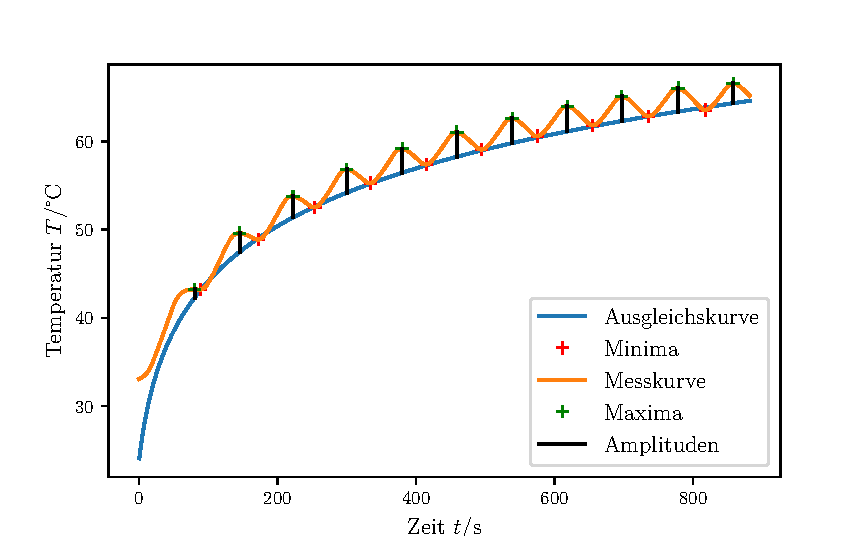
\includegraphics[max width=1.1\linewidth]{plots/amplitudes_brass_wide_far(t1).pdf} %HIER Datei für edelstahl einfügen!
        \caption{T8, fern.}
        \label{fig:plot_amps_t8}
    \end{subfigure}%
    \begin{subfigure}{.5\textwidth}
        \centering
        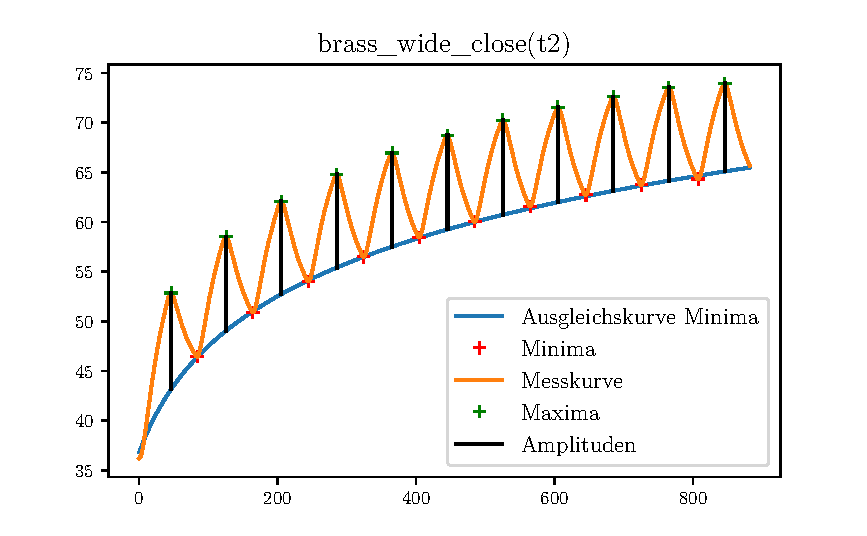
\includegraphics[max width=1.1\linewidth]{plots/amplitudes_brass_wide_close(t2).pdf} %HIER Datei edelstahl einfügen
        \caption{T7, nah.}
        \label{fig:plot_amps_t7}
    \end{subfigure}
    \caption{Messwertanalyse zu Aluminium.}
    \label{fig:plots_amps_t7_t8}
\end{figure}
\begin{table}
    \centering
    \caption{Amplituden von Edelstahl, nah und fern, in $\si{\kelvin}$.}
    \label{tab:amps_steel}
    \begin{tabular}{S[table-format=2.1] | S[table-format=3.1] S[table-format=1.2] | S[table-format=3.1] S[table-format=1.2]}
        \toprule
         & \multicolumn{2}{c}{$\symup{Edelstahl}_\text{nah}$} & \multicolumn{2}{c}{$\symup{Edelstahl}_\text{fern}$} \\
        \cmidrule(lr){2-3}\cmidrule(lr){4-5}
        {$\increment t[\si{\second}]$} &{$t[\si{\second}]$} & {$\increment T[{\si{\kelvin}]}$} & {$t[\si{\s}]$} & {$\increment T[{\si{\kelvin}]}$} \\
        \midrule
        34.0   &  46.5 &	9.70 &    80.5 & 0.91 \\	%hier die Messwerte für edelstahl einfügen (dies sind die von Messing)
        19.5   & 126.0 &	9.47 &   145.5 & 2.11 \\		
        17.0   & 205.5 &	9.36 &   222.5 & 2.39 \\		
        14.5   & 285.5 &	9.38 &   300.0 & 2.63 \\		
        14.5   & 365.5 &	9.43 &   380.0 & 2.72 \\		
        13.5   & 445.5 &	9.46 &   459.0 & 2.78 \\		
        13.5   & 525.5 &	9.53 &   539.0 & 2.81 \\		
        13.5   & 605.0 &	9.57 &   618.5 & 2.84 \\		
        12.0   & 685.0 &	9.47 &   697.0 & 2.78 \\		
        13.5   & 765.0 &	9.40 &   778.5 & 2.65 \\
        \bottomrule
    \end{tabular}
\end{table}
T7, Minima: $\symup{(a,b,c)}=()$ %Parameter für T7 und T8 einfügen
T8, Minima: $\symup{(a,b,c)}=()$
T7, Maxima: $\symup{(a,b,c)}=()$ %Parameter für T7 und T8 einfügen
T8, Maxima: $\symup{(a,b,c)}=()$

\begin{table}
    \centering
    \caption{Edelstahl.}
    \label{tab:unc_steel}
    \begin{tabular}{S S S S S S S S | S S S S S S S S}
        \toprule
        \multicolumn{8}{c}{$\symup{Edelstahl}_\text{nah}$} & \multicolumn{8}{c}{$\symup{Edelstahl}_\text{fern}$} \\
        \cmidrule(lr){1-4}\cmidrule(lr){5-8}\cmidrule(lr){9-12}\cmidrule(lr){13-16}
        {$\increment t_min [\si{\second}]$} & {abgelesene Minima T7} & {$\symup{f_t7(t_min)}$} & {$\increment T_min$} & {$\increment t_max [\si{\second}]$} & {abgelesene Maxima T7} & {\symup{f_t7(t_max)}} & {$\increment T_max$} & 
        {$\increment t_min [\si{\second}]$} & {abgelesene Minima T8} & {$\symup{f_t8(t_min)}$} & {$\increment T_min$} & {$\increment t_max [\si{\second}]$} & {abgelesene Maxima T8} & {\symup{f_t8(t_max)}} & {$\increment T_max$}\\
        \midrule
        %hier entsprechende Zwischenwerte einfügen
        \bottomrule
    \end{tabular}
\end{table}
\begin{table}
    \centering
    \caption{Aus der jeweiligen Messdatenzeile berechnete Wärmeleitfähigkeit $\kappa$.}
    \label{tab:kappa_steel}
    \begin{tabular}{S S}
        \toprule
        {$i$} & {$\kappa_i$} \\
        \midrule
        1 &   \\%hier berechnete werte für kappa einfügen
        2 &   \\
        3 &   \\
        4 &   \\
        5 &   \\
        6 &   \\
        7 &   \\
        8 &   \\
          &   \\
    \end{tabular}
\end{table}
Für die Wärmeleitfähigkeit des Edelstahls ergibt sich an dieser Stelle somit $\kappa = \pm $ %hier kappa für edelstahl einfügen inkl sigma
